\iffalse
Noether's theorem says that continuous symmetries of physical systems gives rise to conservation laws. In this class we'll see some examples of low dimensional Lie groups and how they give rise to various phenomenon in physics like time dilation and length contraction in special relativity, spin states of electrons.

Keywords: bilinear forms, signature, SO(2), SO(3), Spin, SO(1,3), Minkowski space and relativity, Noether's theorem, Lie groups.

Prereqs: Linear algebra, Group theory
Homework: Recommended
\fi



\documentclass{article}
\usepackage{amsmath, amsthm}
\usepackage{amssymb}
\usepackage{mathtools}
\usepackage[all,cmtip]{xy}
\usepackage{color}


\setcounter{tocdepth}{4}

\renewenvironment{proof}{ {\bfseries Proof:}}{\qed}

\newtheoremstyle{mytheorem}%                % Name
{}%                                     % Space above
{}%                                     % Space below
{\itshape}%                                     % Body font
{0pt}%\parindent}%                                     % Indent amount
{\bfseries}%                            % Theorem head font
{.}%                                    % Punctuation after theorem head
{ }%                                    % Space after theorem head, ' ', or \newline
{}%                                     % Theorem head spec (can be left empty, meaning `normal')

\theoremstyle{mytheorem}
\newtheorem{thm}{Theorem}[section]
\newtheorem{proposition}[thm]{Proposition}
\newtheorem{lemma}[thm]{Lemma}
\newtheorem{corollary}[thm]{Corollary}


\newtheoremstyle{mydefinition}%                % Name
{}%                                     % Space above
{}%                                     % Space below
{}%                                     % Body font
{0pt}%\parindent}%                                     % Indent amount
{\bfseries}%                            % Theorem head font
{.}%                                    % Punctuation after theorem head
{ }%                                    % Space after theorem head, ' ', or \newline
{}%                                     % Theorem head spec (can be left empty, meaning `normal')

\theoremstyle{mydefinition}
\newtheorem{definition}[thm]{Definition}
\newtheorem{example}[thm]{Example}
\newtheorem{exercise}[thm]{Exercise}
\newtheorem{remark}[thm]{Remark}
%\newtheorem{ques}[thm]{Q.}
\newtheorem*{ques}{Question}
%\newtheorem{ans}[thm]{Ans.}
\newtheorem*{ans}{Ans}



\numberwithin{equation}{section}

%Real numbers, complex numbers, etc.
\newcommand{\R}{\mathbb{R}}
\newcommand{\C}{\mathbb{C}}
\newcommand{\Z}{\mathbb{Z}}
\newcommand{\Q}{\mathbb{Q}}
\renewcommand{\P}{\mathbb{P}}

%How does latex not have these?
\DeclareMathOperator{\Ad}{Ad}
\DeclareMathOperator{\ad}{ad}
\DeclareMathOperator{\tr}{tr}
\DeclareMathOperator{\Tr}{Tr}
\DeclareMathOperator{\Hom}{Hom}
\DeclareMathOperator{\Spec}{Spec}
\DeclareMathOperator{\im}{im}
\DeclareMathOperator{\rank}{rank}
\DeclareMathOperator{\Exists}{\exists}
\DeclareMathOperator{\Forall}{\forall}

\DeclareMathOperator*{\colim}{colim}
\DeclareMathOperator*{\holim}{holim}
\DeclareMathOperator*{\hocolim}{hocolim}


%fractions and inner product
\newcommand{\pr}[2][\:]{\frac{\partial #1}{\partial #2}}
\newcommand{\innerp}[2]{\langle #1, #2 \rangle}

\newcommand*\conj[1]{\overline{#1}}
\newcommand*\norm[1]{\lVert #1 \rVert}

\renewcommand{\figurename}{Fig.}
\usepackage{float}
\usepackage{wrapfig}

\usepackage{enumitem}
\setlist[enumerate]{itemsep=0mm}
\usepackage{geometry}
\geometry{
	a4paper,
	total={170mm,257mm},
	left=20mm,
	top=20mm
}


\usepackage{fancyhdr}
\pagestyle{fancy}
\lhead{\scshape Apurva Nakade}
%\rhead{\scshape Mathcamp 2017}
\renewcommand*{\thepage}{\small\arabic{page}}

\DeclareMathOperator{\re}{Re}



\begin{document}
\title{Inverses of polynomials}
\author{Apurva Nakade}
\thispagestyle{fancy}
\maketitle




Today's goal is to build Riemann surfaces on which inverses of polynomials $f(z)$ can be well defined.

\section{Riemann surface for $\log z$}
If we try to define $\log z$ naively using polar coordinates we get
\begin{align}
	\log (re^{i \theta}) & = \log r + i \theta
\end{align}
We have a discontinuity at $\theta = 0$ and $\theta = 2 \pi$ so we need to make a branch cut, say at $\theta = 0$, to get a well defined function. For $\theta$ varying in the range $(0,2\pi)$ we get one branch function. We get other (distinct) branches by adding multiples of $2 \pi$ to $\theta$.
\begin{align}
	\log (re^{i \theta}) & = \log r + i (\theta + 2 n \pi)
\end{align}
To create a Riemann surface on which $\log z$ is well defined we need $\Z$ many copies of $\C$, on which we make branch cuts and glue them together.




\section{Winding numbers}
In order to generalize the above situation to more complicated functions we analyze what is happening here. For this we need the notions of winding numbers.

Consider a non-constant complex differentiable function $f:\C \rightarrow \C$. Fix a point $p \in \C$ be a complex number. Let $\gamma:[0,2\pi] \rightarrow \C$ with $\gamma(0) = \gamma(2\pi)$ be an embedded loop in $\C$ (no self intersections) containing $p$ in it's interior that goes counterclockwise. We say that $\gamma$ is \textbf{sufficiently close} to $p$ if there are no points $p' \neq p$ in the interior of $\gamma$ such that $f(p) = f(p')$.

\begin{proposition}
	For all points $p \in \C$ there exists a loop $\gamma$ sufficiently close to $p$.
\end{proposition}
\begin{proof}
	Consider the function $g(z) = f(z) - f(p)$. The zeroes of this complex differentiable function are exactly the points $p'$ such that $f(p') = f(p)$. Complex differentiable functions have isolated zeroes and hence $p$ has a neighborhood $U$ which does not contain any other zero of $g$. Any loop $\gamma$ in $U$ is sufficiently close to $p$.
\end{proof}


\begin{definition}
	Let $\gamma$ be a loop sufficiently close to $p$. The composition $f \circ \gamma$ is a loop around $f(p)$ (not necessarily embedded). The \textbf{winding number} $w_f(p)$ is the number of counterclockwise revolutions made by $f \circ \gamma$ around $f(p')$ minus the number of clockwise revolutions.
\end{definition}

\begin{proposition}
	Without any loss of generality assume that $p=0$ and $f(p) = 0$. Let $\gamma(t)$  be a loop sufficiently close to $p$ then the winding number is given by
	\begin{align}
		\label{eq:winding}
		w_f(0) & = \dfrac{\log(f ( \gamma(2 \pi))) - \log(f ( \gamma(0)))}{2 \pi i}
	\end{align}
	where $\log(z)$ is any branch of the logarithm.
\end{proposition}
\begin{proof}
	For every single counterclockwise revolution $\log(z)$ increases by $2 \pi i$ and for every single counterclockwise revolution $\log(z)$ decreases by $ 2 \pi i$. The result follows.
\end{proof}

\begin{example}
	For the function $f(z) = z^n$ the winding number around 0 is $n$ and the winding number around $p \neq 0$ is 1.
\end{example}



\subsection{Points with winding number $> 1$}
For the function $z^n$ the only complex number $z$ for which the winding number is bigger than 1 is $z=0$ and this is the point where we've to make a branch cut. This suggests that to define inverses of more complicated functions we need to figure out the points at which the winding number is greater than 1.

Let $f(z)$ be a complex differentiable function. Consider a point $p \in \C$ and let $f(z) = \sum \limits_{i=0}^\infty a_i (z-p)^i$ be the Taylor series of near $p$.

\begin{proposition}
	\label{thm:windingNum}
	The winding number of $w_f(p)$ is the smallest non-zero integer $i$ such that $a_i \neq 0$.
\end{proposition}
\begin{proof}
	By shifting origin if necessary assume that $p=0$ and $f(p) = 0$ so that the Taylor expansion looks like $$f(z) = \sum \limits_{i=n}^\infty a_i z^i = z^n \sum \limits_{i=n}^\infty a_i z^{i-n} = z^n g(z) $$ for some $n > 0$ where $a_n \neq 0$ and $g(z) = \sum \limits_{i=n}^\infty a_i z^{i-n}$. The function $g(z)$ has the property that $g(0) \neq 0$. If we choose a loop $\gamma$ sufficiently close to $0$ such that $g(\gamma(t))$ stays very close to $g(0)$ then $g(z)$ is almost constant non-zero number and hence the winding number $w_f(p) = w_{z^n}(p)$ which equals $n$.
\end{proof}

With this proposition the points with winding number bigger than 1 are easily determined.
\begin{cor}
	$w_f(p) > 1$ iff $f'(p) = 0$ i.e. the points with winding number bigger than 1 are exactly the critical points of $f$.
\end{cor}


\section{Covering spaces}
Consider the function $f(z) = z^n$. For any non-zero $p$ the set $f^{-1}(p)$ contains exactly $n$ elements $p_1, \cdots, p_n$. More is true, there exists a neighborhood $U \ni p$ such that $f^{-1}(U)$ is isomorphic to $n$ non-intersecting neighborhoods of the $n$ points $U_1 \ni p_1, \cdots, U_n \ni p_n$. Furthermore the restriction of the map $f|_{U_i}$ is an isomorphism\footnote{homeomorphism}. These properties define what is called a covering space.

\begin{definition}
	A map $p: X \rightarrow Y$ is a \textbf{covering map} if for every point $y \in Y$ there exists a neighborhood $U \ni y$ such that
	\begin{enumerate}
		\item $p^{-1}(U)$ is a disjoint union of subsets $\{ V_i \}_{i \in I}$ of $X$ for some indexing set $I$
		\item The restriction $p|_{V_i} : V_i \rightarrow U$ is an isomorphism for each $i \in I$.
	\end{enumerate}
	$X$ is called a \textbf{covering space} of $Y$.\\
\end{definition}

\begin{center}
	\begin{tabular}{ccc}
		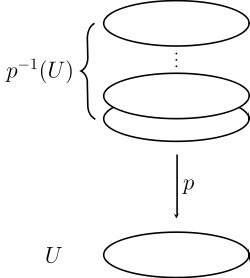
\includegraphics[width=0.35\linewidth]{images/covering_space} & $\qquad \qquad$ &
		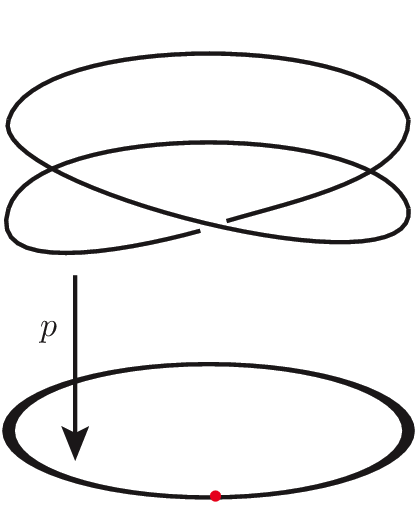
\includegraphics[width=0.25\linewidth]{images/branched_covering_space} \\
		$\qquad \qquad \qquad$ Covering Space                         &                 & Branched Covering Space
	\end{tabular}
\end{center}


So the map $z^n : \C \setminus \{ 0\} \rightarrow \C \setminus \{ 0 \}$ is a covering map. A map which is a covering map at all points except some isolate ones is called a \textbf{branched covering}. So $z^n: \C \rightarrow \C$ is a branched covering.

More generally every complex differentiable function $f(z):\C \rightarrow \C$ is a branched covering and it's restriction to the complement of critical points of $f(z)$ is a covering map.

\subsection{Monodromy}
Consider again the function $z^n: \C \rightarrow \C$. Consider a loop around the origin in the \textbf{target} complex plane passing through $z=1$. If we traverse the loop once and try to lift the loop back up to the domain $z$ then the loop does not remain a loop but becomes a path connecting 1 to the root of unity $e^{2 \pi i/n}$. In this we say that the covering $z^n$ has non-trivial \textbf{monodromy}. Monodromy is the mathematical reason why need to glue complex planes to create Riemann surfaces.\footnote{There is in fact a monodromy group that is acting upon the various sheets via permuting them.}



\subsection{Constructing the Riemann surface}

So the strategy to define the inverse of a polynomial $f(z)$ is the following:
\begin{enumerate}
	\item Find the critical points of $f(z)$
	\item On the non-critical points $f(z)$ is a covering map, find the number of \emph{sheets} over each point using winding numbers
	\item Make branch cuts at each critical point and glue the sheets of complex plane to get a Riemann surface.
\end{enumerate}




\section{Exercises}

\begin{exercise}
	Show that the winding number of $f(z) = z^n$ at $p \in \C$ is equal to
	\begin{align}
		w_f(p) = \dfrac{1}{2 \pi i} \int_{\gamma} \dfrac{f(z)}{(z-p)^{n+1}} dz
	\end{align}
	$\gamma$ is a loop sufficiently close to $p$.

	Prove this formula for an arbitrary complex differentiable function $f(z)$.
\end{exercise}


\begin{exercise}
	Fill in the gaps in the proof of Proposition \ref{thm:windingNum}.
\end{exercise}


\begin{exercise}
	Construct Riemann surfaces for the following polynomials:
	\begin{enumerate}
		\item $f(z) = z^2 - 2 z$
		\item $f(z) = z^3 - 3z$
	\end{enumerate}
\end{exercise}


\end{document}
